\documentclass[tikz,border=2pt]{standalone}
\usepackage{amsmath}
\usetikzlibrary{arrows.meta}
\begin{document}
% Outside option followed by a simultaneous game: the singleton node after In starts a subgame
% that contains both nodes of player 2's information set; player 2's nodes cannot start a
% subgame. Together with the whole game there are 2 subgames.
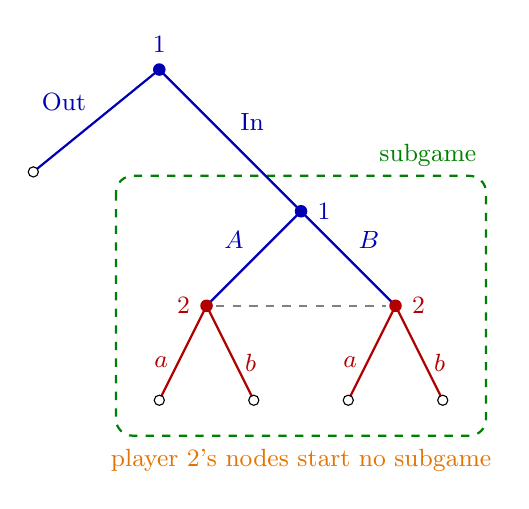
\begin{tikzpicture}[font=\small, >={Latex[length=2mm]},
    dec/.style={circle, fill, inner sep=1.6pt},
    term/.style={circle, draw, fill=white, inner sep=1.3pt}]
  % subgame starting after In
  \draw[green!50!black, dashed, thick, rounded corners=6pt] (-0.55,-0.95) rectangle (4.15,-4.25);
  \node[green!50!black, anchor=south east] at (4.15,-0.95) {subgame};
  % edges
  \draw[thick, blue!70!black] (0,0.4) -- node[above left, pos=0.5] {Out} (-1.6,-0.9);
  \draw[thick, blue!70!black] (0,0.4) -- node[above right, pos=0.5] {In} (1.8,-1.4);
  \draw[thick, blue!70!black] (1.8,-1.4) -- node[above left, pos=0.5] {$A$} (0.6,-2.6);
  \draw[thick, blue!70!black] (1.8,-1.4) -- node[above right, pos=0.5] {$B$} (3.0,-2.6);
  \draw[thick, red!70!black] (0.6,-2.6) -- node[left, pos=0.6] {$a$} (0.0,-3.8);
  \draw[thick, red!70!black] (0.6,-2.6) -- node[right, pos=0.6] {$b$} (1.2,-3.8);
  \draw[thick, red!70!black] (3.0,-2.6) -- node[left, pos=0.6] {$a$} (2.4,-3.8);
  \draw[thick, red!70!black] (3.0,-2.6) -- node[right, pos=0.6] {$b$} (3.6,-3.8);
  % player 2's information set
  \draw[dashed, thick, gray] (0.72,-2.6) -- (2.88,-2.6);
  % nodes
  \node[dec, blue!70!black, label={[blue!70!black]above:$1$}] at (0,0.4) {};
  \node[dec, blue!70!black, label={[blue!70!black]right:$1$}] at (1.8,-1.4) {};
  \node[dec, red!70!black, label={[red!70!black]left:$2$}] at (0.6,-2.6) {};
  \node[dec, red!70!black, label={[red!70!black]right:$2$}] at (3.0,-2.6) {};
  \foreach \x/\y in {-1.6/-0.9, 0.0/-3.8, 1.2/-3.8, 2.4/-3.8, 3.6/-3.8} \node[term] at (\x,\y) {};
  % player 2's nodes start no subgame
  \node[orange!90!black, anchor=north] at (1.8,-4.3) {player $2$'s nodes start no subgame};
\end{tikzpicture}
\end{document}
